\chapter{Finite State Machines (FSMs)}
\label{ch:fsm}

\section{What is a finite state machine?}
A \textbf{finite state machine} is a simple but powerful way to model a process that moves through
a limited number of situations (called \textbf{states}) based on events or inputs (called \textbf{symbols}).

At any moment:
\begin{itemize}
  \item the machine is in \textbf{exactly one state},
  \item it receives an \textbf{input event} (or a timer tick, or a button press, etc.),
  \item it follows a \textbf{transition} to the next state,
  \item and (optionally) it produces an \textbf{output/action}.
\end{itemize}

A common formal definition (for a deterministic finite automaton, DFA) is the 5-tuple
$(Q, \Sigma, \delta, q_0, F)$:
\begin{itemize}
  \item $Q$ = set of states
  \item $\Sigma$ = input alphabet (the set of possible events)
  \item $\delta$ = transition function ($Q \times \Sigma \to Q$)
  \item $q_0$ = start state
  \item $F$ = set of accepting/terminal states (optional for many programming-style FSMs)
\end{itemize}

In software engineering, we often use FSMs without emphasizing ``accepting states''---instead we care about:
\textbf{valid transitions}, \textbf{illegal transitions}, and how to implement the state logic cleanly.

% Optional citations (add to references.bib if you use these)
% \cite{sipser_toc,hopcroft_automata}

\section{Warm-up example 1: traffic light}
Before we touch Monty Hall, here is a classic FSM: a traffic light.
It has a tiny state set, clear transitions, and it’s easy to test.

\begin{figure}[h!]
  \centering
  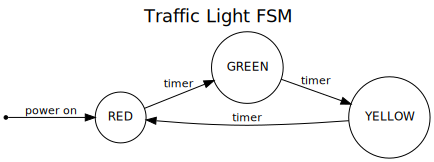
\includegraphics[width=0.72\linewidth]{traffic_light_fsm.pdf}
  \caption{A simple traffic light FSM.}
  \label{fig:traffic-light-fsm}
\end{figure}

\section{Warm-up example 2: turnstile (coin / push)}
Another famous teaching FSM is a subway turnstile.
Important lesson: \textbf{the same input can have different effects depending on the current state}.
That’s the entire point of state.

\begin{figure}[h!]
  \centering
  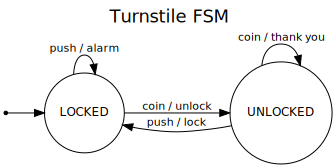
\includegraphics[width=0.78\linewidth]{turnstile_fsm.pdf}
  \caption{Turnstile FSM: locked/unlocked behavior.}
  \label{fig:turnstile-fsm}
\end{figure}

\section{Warm-up example 3: login session / lockout}
FSMs also show up everywhere in security and application UX.
A login flow is a state machine: logged out, authenticating, logged in, locked out, etc.

\begin{figure}[h!]
  \centering
  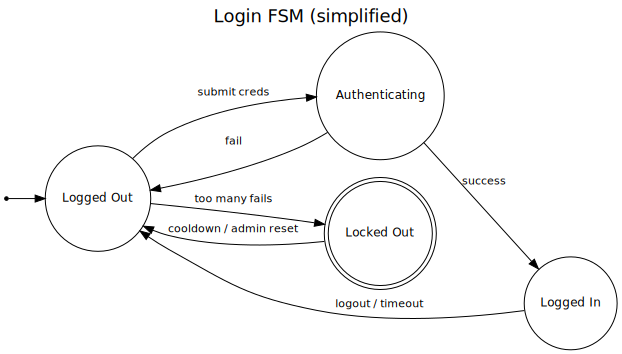
\includegraphics[width=\linewidth]{login_fsm.pdf}
  \caption{A simplified login FSM with lockout.}
  \label{fig:login-fsm}
\end{figure}

\section{How FSMs map to code (the practical part)}
In code, an FSM usually becomes:
\begin{itemize}
  \item an \texttt{enum} (or strings) representing states,
  \item an ``event'' type (another enum or strings),
  \item a transition function: \texttt{(state, event) -> new\_state},
  \item optional actions performed on transitions.
\end{itemize}

This approach gives you three superpowers:
\begin{enumerate}
  \item \textbf{Clarity:} you can explain behaviour with a diagram.
  \item \textbf{Testability:} you can unit-test every transition and every illegal move.
  \item \textbf{Instrumentation:} you can log events and states to produce clean datasets.
\end{enumerate}

\section{Deterministic vs.\ nondeterministic (and why we mostly use deterministic in software)}
A \textbf{deterministic} FSM has at most one outgoing transition per input symbol from each state.
A \textbf{nondeterministic} FSM can have multiple possible next states for the same input.
In programming projects like ours, we typically build deterministic FSMs, then model randomness as:
\begin{itemize}
  \item probabilistic choices (e.g., random door placement),
  \item or hidden variables (car door, chosen door),
  \item or both.
\end{itemize}

When an FSM includes variables (like ``car\_door'' or ``player\_choice''), many people call it an
\textbf{extended finite state machine (EFSM)}: the state diagram is still the backbone, but we track
a few additional values to make the model realistic.

\section{The Monty Hall FSM (our blueprint)}
Now we apply the same idea to the Monty Hall game.
We will refine and expand this FSM as needed, but the key stages are:
\textbf{setup} $\rightarrow$ \textbf{player picks} $\rightarrow$ \textbf{host reveals} $\rightarrow$
\textbf{player decides} $\rightarrow$ \textbf{resolve} $\rightarrow$ \textbf{reset}.

\begin{figure}[h!]
  \centering
  \includegraphics[width=\linewidth]{monty_hall_fsm_diagram.pdf}
  \caption{Monty Hall FSM (Graphviz-generated).}
  \label{fig:monty-hall-fsm}
\end{figure}

\section{Where we go next}
In Chapter 3, we design a data-collection FSM that formalizes \emph{exactly} how simulation trials run,
what gets logged, and how results flow into tables and plots.
That design becomes the contract for the code and the unit tests.

